
The goal of our work is to extract opinions and sentiments about mobile applications from user reviews written in Thai. The work hopes to help Thai users assess mobile applications without needing to read all reviews and to also help Thai developers pinpoint where they can improve their software products. To achieve the goal, we employ 5 steps, shown in Figure \ref{fig:approachFig}, as follows: 1. Data Collection 2. Prepossessing 3. Sentiment Analysis 4. Topic Extraction 5. Summary. 

\begin{figure}[t]
	\centering
	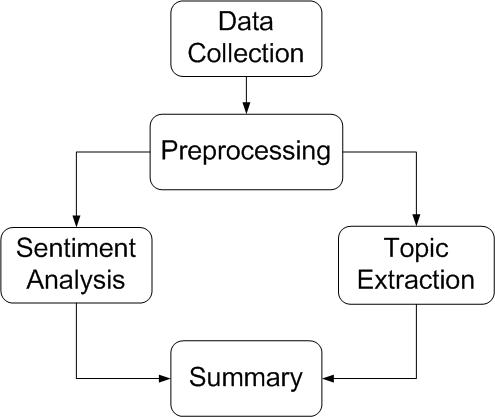
\includegraphics[width=.5\linewidth]{Process.jpg}
	\caption{Overview of our approach}
	\label{fig:approachFig}
\end{figure}

We would like the entire process to be as automatic and accurate as possible, but there are several limitations. To process raw user reviews, most of the process can be done automatically but some steps need manual intervention. Following subsections describes these five steps and also states whether the step is done automatically or manually. We also make an assumption that one sentence has one sentiment to make the process possible. 

\subsection{Data Collection}

\begin{table}[h]
	\caption{Number of reviews in each application}
	\label{table:NoOfReview}
	\centering
	\begin{tabular}{|c|r|}
		\hline
		\textbf{Application} & \multicolumn{1}{|c|}{\textbf{No. of Reviews}} \\
		\hline
		Man Man & 1,279\\
		\hline
		H-TV & 691\\
		\hline
%		K-Mobile & 1,055\\
%		\hline
	\end{tabular}
\end{table}

\begin{table*}[h]
	\caption{Example of Reviews}
	\label{table:review}
	\centering
	\begin{tabular}{|l|l|l|c|c|}
		\hline
		\multicolumn{1}{|c|}{\textbf{Author}} &
		\multicolumn{1}{|c|}{\textbf{Title}} &
		\multicolumn{1}{|c|}{\textbf{Review}} &
		\multicolumn{1}{|c|}{\textbf{Rate}} &
		\multicolumn{1}{|c|}{\textbf{Date} (mm/dd/yyyy)}\\
		\hline
		{\selectlanguage{thai}โชคชัย มหาวงนันท์} & {\selectlanguage{thai}โชคชัย มหาวงศ์นันท์} & {\selectlanguage{thai}ใช้ได้ดีครับ} (works good.) & 5&10/04/2015\\
		\hline
		bie slow life &  & {\selectlanguage{thai}พักหลังนี่อัพบ่อยนะครับ} (Later, frequently update.) & 4&09/19/2015\\
		\hline
		ornanohg Hongrrimon &  & {\selectlanguage{thai}ชอบค่ะใช้ง่าย มีตัวการ์ตูนให้ด้วย} (like it. easy to use, have sticker) & 5&09/20/2015\\
		\hline
		Terdsak chompusri &  & {\selectlanguage{thai}เรียบง่ายแต่ใช้ได้ดีจริงๆครับชอบมาก} (Simple but really works good. Like it.) & 5&09/22/2015\\
		\hline
		Worapote Panomauppatum & {\selectlanguage{thai}วรพจน์  พนมอุปถัมภ์} & {\selectlanguage{thai}ใช้ได้เยื่ยมมาก} (Very good) & 5&09/25/2015\\
		\hline
		Nate Makboon & {\selectlanguage{thai}เนตร มากบุญ} & {\selectlanguage{thai}ดีมากครับ สะดวกดีแม่นสุดยอด} (Very good. comfortable and accurately) & 5&09/24/2015\\
		\hline
	\end{tabular}
\end{table*}


We collected user reviews in Google Play Store from two mobile applications:
\enquote{{\selectlanguage{thai}แม่น แม่น}} or \enquote{Man Man} (a virtual keyboard) and \enquote{H-TV} (online TV). The user reviews collected are dated between February 2015 and August 2016. The number of user reviews for each application is shown in Table \ref{table:NoOfReview}. The information for each review includes author, title, detail, rate, and review date. Table \ref{table:review} shows examples of user reviews. 

The collection process is done automatically using JavaScript to retrieve user reviews automatically from the Google Play Store website. The user reviews are then stored in a database for further analysis.

\subsection{Prepossessing}

After user reviews have been collected, the next step is to perform sentence segmentation, word segmentation and part-of-speech tagging. 

\subsubsection{sentence segmentation}
One user review can contain several sentences expressing opinions about various aspects. 
Since we make an assumption that one sentence has one sentiment, we need to break reviews into a list of single sentences. Thai writing makes it difficult because there is no formal sentence boundary like a period or a question mark in Engish. Spaces in Thai can mark the end of a sentence or the end of a clause. Therefore, we cannot simply use spaces to indicate the end of sentences. Although there are several researches focusing on breaking Thai text into sentences, there are no tools that can easily be used. We therefore perform sentence segmentation manually. Once a tool is available, it can be applied to make this pre-processing step easier. 

\subsubsection{word segmentation}
As mentioned in Section \ref{Background}, we use LexTo\cite{LexTo} from NECTEC to perform word segmentation. LexTo can segment words very well if words are spelled correctly. However, processing raw user reviews is difficult because of the informal language and slangs used in the reviews. There are also many spelling errors, either accidentally or intentionally to emphasize the meaning such as \enquote{{\selectlanguage{thai}มากกกกกก}}, causing the tool to segment words incorrectly. 

%To ease the problem, LexTo allows us to add new vocabulary into the tool. However, with too many slangs including new ones and too many variations of misspelled words, it is not practical to add all of these into the tool. Today, more and more texts to be analyzed are written informally. It is more practical to find an automatic approach to deal with this problem rather than manually correctly these words so that the word segmentation tool can perform entirely correctly. In our work, we have added some common slangs and common misspelled into the tool to increase accuracy but are not able to cover all slangs and mispelled words. This step is therefore more automatic with the cost of less accuracy.

Today, more and more texts are written informally. It is not practical to manually correct these words so that the word segmentation tool can perform correctly. In our work, we want this step to be automatic and therefore, we sacrifice accuracy. 

%we have added some common slangs and common misspelled into the tool to increase accuracy but are not able to cover all slangs and mispelled words. This step is therefore more automatic with the cost of less accuracy.

\subsubsection{POS tagger}

We use the RDRPOStagger tool\cite{RDRPOSTagger} with the ORCHID corpus\cite{ORCHID} for POS tagging. Since some slang and misspelled words are segmented incorrectly, the POS tool tags those words as \enquote{unknown}. In the sentiment analysis and topic modeling steps, only words tagged with nouns, verbs, and adjective/adverb are used. Moreover, since one word can be tagged with more than one POS, this POS annotation is used to identify various meanings of one word. For example, the word \enquote{{\selectlanguage{thai}ฉัน}} has two meanings with different parts of speech. As a noun, it means \enquote{I}. As a verb, it means \enquote{eat}.

\subsection{Sentiment Analysis}
Once words in user reviews are tagged with POS, sentiments in these reviews can be analyzed. Our work applies the lexicon-based approach. However, there is no resource that annotates each Thai word with sentiment scores. Therefore, the English SentiWordNet \cite{SentiWordNet} is used in combination with an electronic Thai-English dictionary called LEXiTRON \cite{LEXiTRON} developed by NECTEC. Note that some words in the reviews are already written in English. For these English words, their sentiment scores can be retrieved from SentiWordNet without using LEXiTRON.

We assign sentiment scores only to words tagged with nouns, verbs, and adjective/adverb. To find score for each of these Thai words, our script automatically looks up in the LEXiTRON dictionary to retrieve its English translation with the same POS. The next step is to look for sentiment scores in SentiWordNet for the English word with the same POS. In SentiWordNet, each word is assigned with three numerical scores: \textit{Pos}, \textit{Neg}, \textit{Obj}. These numbers indicate how positive, negative, and \enquote{objective} (or neutral) the word is where each number is between [0.0,1.0] and their sum is 1.0. In our approach, we assign only one numerical score to a word by subtracting the \textit{Neg} score from the \textit{Pos} score. Since \textit{Obj} means neutral, we do not take this number into account.  

Moreover, further analysis is also needed. For example, a word preceded with {\selectlanguage{thai}ไม่}, which means \enquote{no} or \enquote{not}, will have its sentiment score reversed. In addition, some Thai words have more than one associated English translations with the same POS which have different sentiment scores. Some Thai words may have more than one associated English translations but none has the same POS. In both cases, all sentiment scores from all translations are averaged and then assigned to the Thai word. Table \ref{table:Top10sentiword} shows top ten words for each sentiment found in user reviews from Man Man application. 

\begin{table}[h]
	\renewcommand{\arraystretch}{1.3}
	\caption{Top 10 words for each sentiment in Man Man application}
	\label{table:Top10sentiword}
	\centering
	\begin{tabular}{|l|c|l|c|}
		\hline
		\multicolumn{2}{|c|}{\textbf{Negative}} &
		\multicolumn{2}{|c|}{\textbf{Positive}} \\
		\hline
		\textbf{\textit{Word}} & \textbf{\textit{Sentiment}} & \textbf{\textit{Word}} & \textbf{\textit{Sentiment}}\\
		\hline
		{\selectlanguage{thai}ลบ} (delete) & -0.33621 & {\selectlanguage{thai}น่ารัก} (cute) & 0.21843\\
		\hline
		{\selectlanguage{thai}เสียดาย} (deplore) & -0.17095 & {\selectlanguage{thai}รัก} (love) & 0.20107\\
		\hline
		{\selectlanguage{thai}เกลียด} (hate) & -0.16666 & {\selectlanguage{thai}เพลิน (enjoy*)} & 0.17563\\
		\hline
		{\selectlanguage{thai}ดุ} (fierce) & -0.15297 & {\selectlanguage{thai}ดี} (good) & 0.16622\\
		\hline
		{\selectlanguage{thai}สายตายาว} (presbyopia) & -0.12500 & {\selectlanguage{thai}สวย} (beautiful) & 0.16310\\
		\hline
		{\selectlanguage{thai}ขยายตัว (expand)} & -0.09566 & {\selectlanguage{thai}สุดยอด} (topmost) & 0.15476\\
		\hline
		{\selectlanguage{thai}ห่วย} (bad) & -0.09071 & {\selectlanguage{thai}มันส์} (enjoy*) & 0.15085\\
		\hline
		{\selectlanguage{thai}ปวด} (pain) & -0.07943 & {\selectlanguage{thai}ไว} (fast) & 0.12500\\
		\hline
		{\selectlanguage{thai}เสียใจ} (sad) & -0.07943 & {\selectlanguage{thai}ชอบ} (like) & 0.12246\\
		\hline
		{\selectlanguage{thai}ไม่ดี} (not good) & -0.06995 & {\selectlanguage{thai}สนุก (amuse, enjoy)} & 0.10604\\
		\hline
	\end{tabular}
\end{table}


When sentiment scores are assigned to all nouns, verbs, adjectives, and adverbs in a sentence, the sentiment score for the sentence is calculated by averaging these sentiment scores. 

Furthermore, we find that several negative sentences are assigned with positive score. Upon closer look, we find a pattern in these sentences where there is a word {\selectlanguage{thai}ชอบ} preceding with a negative verb such as \enquote{{\selectlanguage{thai}ชอบค้างบ่อยๆ}}, which means the application often freezes. The word {\selectlanguage{thai}ชอบ} in Thai means \enquote{like}, and if used in front of a verb, it also means \enquote{often}. Since the POS tool tags {\selectlanguage{thai}ชอบ} as a verb which associates with the \enquote{like} meaning, its sentiment score is returned with a high positive number. This type of sentences is therefore incorrectly assigned with positive sentiment. Hence, we eliminate the word {\selectlanguage{thai}ชอบ} that precedes a verb to increase accuracy.

\subsection{Topic/Aspect Extraction}
In addition to sentiment analysis, we also want to pinpoint what aspects users are talking about in the reviews. We use LDA, a topic modeling technique, to extract topics/aspects. We supply only nouns, verbs, adjectives, and adverbs in all user reviews to the LDA Python tool. 

When using the LDA technique, a number of topics must be specified. Since we do not know exactly how many aspects users are talking about in the reviews, we have experimented on different numbers of topics ranging from 10, 11, ..., 20. We find that main topics stay put when increasing the number of topics and as the number of topics gets higher, the more refined topics seem to be. We then choose the number of topics to be 20 so that it is not too few nor too many to comprehend the information. To make this process more flexible, we can make this number of topics configurable.

After running LDA, for each topic, several words and associated probabilities that the words belong that topic are returned. LDA does not return the \enquote{name} of the topic. Thus, to interpret the LDA result, we manually choose a few words with high probabilities as the name of the topic/aspect so that users and developers can easily understand results.

\subsection{Summary}
\label{Summary}
After sentences are annotated with sentiment scores and aspects are extracted, we summarize the information by assigning sentiment scores to the extracted aspects. The assigning process is done as follows. For each word belonging in a topic, we find all the sentences containing the word and collect all their sentiment scores. The absolute maximum sentiment score is then assigned to the topic.

In addition, we also count how many sentences with positive and negative sentiments for each topic so that developers can see in more details how much users like or dislike the aspects. 


